% -*- TeX:de -*-
\NeedsTeXFormat{LaTeX2e}
\documentclass[12pt,a4paper]{article}
\usepackage[german]{babel} % german text
\usepackage[DIV12]{typearea} % size of printable area
\usepackage[T1]{fontenc} % font encoding
%\usepackage[latin1]{inputenc} % most likely on Windows
\usepackage[utf8]{inputenc} % probably on Linux
\usepackage{multicol}

% PLOTTING
\usepackage{pgfplots} 
\usepackage{pgfplotstable}

\usepackage{graphicx} % to include images
\usepackage{tikz}
\usepackage{subfigure} % for creating subfigures
\usepackage{amsmath} % a bunch of symbols
\usepackage{amssymb} % even more symbols
\usepackage{booktabs} % pretty tables

% a floating environment for circuits
\usepackage{float}
\usepackage{caption}

%\newfloat{circuit}{tbph}{circuits}
%\floatname{circuit}{Schaltplan}

% a floating environment for diagrams
%\newfloat{diagram}{tbph}{diagrams}
%\floatname{diagram}{Diagramm}

\selectlanguage{german} % use german

\begin{document}

%%%%%%% DECKBLATT %%%%%%%
\thispagestyle{empty}
			\begin{center}
			\Large{Fakultät für Physik}\\
			\end{center}
\begin{verbatim}


\end{verbatim}
							%Eintrag des Wintersemesters
			\begin{center}
			\textbf{\LARGE WS 2013/14}
			\end{center}
\begin{verbatim}


\end{verbatim}
			\begin{center}
			\textbf{\LARGE{Physikalisches Praktikum\\ für das Bachelorstudium}}
			\end{center}
\begin{verbatim}




\end{verbatim}

			\begin{center}
			\textbf{\LARGE{PROTOKOLL}}
			\end{center}
			
\begin{verbatim}





\end{verbatim}

			\begin{flushleft}
			\textbf{\Large{Experiment (Nr., Titel):}}\\
							%Experiment Nr. und Titel statt den Punkten eintragen
			\LARGE{PW1, Messen - Messfehler}	
			\end{flushleft}

\begin{verbatim}

\end{verbatim}	
							%Eintragen des Abgabedatums, oder des Erstelldatums des Protokolls
			\begin{flushleft}
			\textbf{\Large{Datum:}} \Large{17.10.2013}
			\end{flushleft}
			
\begin{verbatim}
\end{verbatim}
							%Namen der Protokollschreiber
		\begin{flushleft}
			\textbf{\Large{Namen:}} \Large{Patrick Braun, Johannes Kurz}
			\end{flushleft}

\begin{verbatim}


\end{verbatim}
							%Kurstag und Gruppennummer, zb. Fr/5
			\begin{flushleft}
			\textbf{\Large{Kurstag/Gruppe:}} \Large{DO/2}
			\end{flushleft}

\begin{verbatim}



\end{verbatim}
							%Name des Betreuers, das Praktikum betreute.
			\begin{flushleft}
			\LARGE{\textbf{Betreuer:}}	\Large{Johanna Akbarzadeh}	
			\end{flushleft}

%%%%%%% DECKBLATT ENDE %%%%%%%
\pagebreak
\setlength{\columnsep}{20pt}
\begin{multicols}{2}
\section{Einleitung}
In diesem (ersten) Praktikumsbeispiel geht es um Messen, Messfehler und -unsicherheiten.
Da Messung ein (wenn nicht "der") Bestandteil eines jeden Experimentes ist, ein Thema, das sich durch alle Bereiche, nicht nur der Physik zieht, steht diese Aufgabenstellung am Anfang des Anfängerpraktikums und ist aufgeteilt auf 3 kleinere Beispiele aus unterschiedlichen Bereichen:\\
\textbf{Längenmessung:} die Stärke eines Kupferdrahtes wurde mittels unterschieldicher Methoden gemessen\\
\textbf{Zeitmessung und Unsicherheit:} die Bestimmung der Gravitationsbeschleunigung durch die Schwingungsdauer eines Fadenpendels\\
\textbf{Spannung/Strom:} Bestimmung von Widerständen durch die Messung von Strom und Spannung in einfachen Netzwerken\\
\\
Neben dem Titel der Einheit, ist den Beispielen eine Einführung in verschiedene grundlegende Messgeräte gemeinsam, sowie erste Erfahrungen im Aufbau einfacher Experimente, gleichzeitiger erster on-the-fly-Überprüfungen der gemessenen Werte sowie Fehlerminimierung.\\
\\
Aufgrund der Struktur der Praktikums-Einheit, ist also auch dieses Protokoll in 3 Teilen gegliedert:\\
TODO 1\\
TODO 2\\
TODO 3\\

\section{Einfache mechanische Messungen}
\subsection{Bestimmung der Dicke eines Kupferdrahtes (und ein Dreieck)}
\begin{figure}[H]
	\centering
  	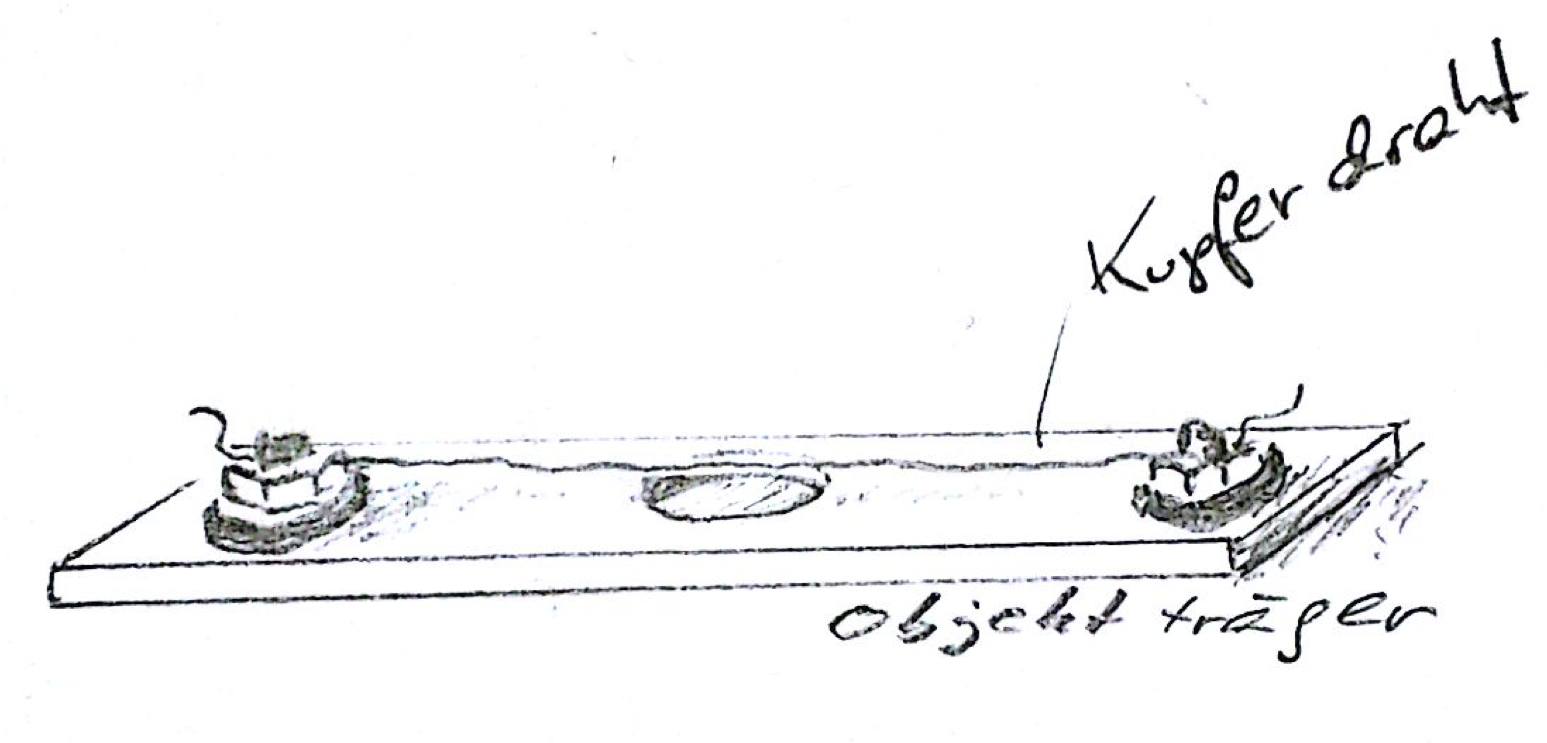
\includegraphics[scale=0.3]{./figure/draht.png}
	\caption{Drahtprobe auf Objektträger}
	\label{fig:101}
\end{figure}
In diesem Beispiel soll die Stärke eines dünnen Kupferdrahtes, an verschiedenen Stellen, mit 3 unterschiedlichen Geräten bestimmt werden: mittels Schieblehre, Mikrometerschraube und der Okularskala in einem Mikroskop.\\
Dabei soll zum einen der Umgang mit diesen Messgeräten grundlegend erlernt und geübt, die Messunsicherheiten, Fehlerquellen, Vor- und Nachteile der einzelnen Geräte erkundet, sowie vergleichende Betrachtungen der (zu erwartenden) unterschiedlichen Ergebnissen aller 3 Methoden erarbeitet werden.\\
Zusätzlich sollen auch die Winkel eines Metall-Dreiecks mit einer Winkellehre gemessen werden, und die Ergebnisse mit deren zu erwartender Summe verglichen werden.\\
\\
Es steht also weniger das Messergebnis selbst (also die Dicke des Drahtes) im Fokus dieser Arbeit, sondern die verschiedenen Wege, die zu diesem führen.\\
Es ist sowohl mit verschiedensten Fehlern und Fehlerquellen zu rechnen, die im Folgenden diskutiert werden, sowie mit Messunsicherheiten, die, abhängig von der jeweiligen Messmethode und deren Auflösung, verschieden groß sind. Außerdem soll in der Diskussion des Experiments auch die Anwendbarkeit und Praktikabilität der Messgeräte im Bezug auf eben unser Beispiel, die Kupferdrahtdicke, besprochen werden.\\
\\

\subsection{Der Aufbau und der Versuch}
%%%% MESSUNGEN
%\subsection{Messung der Dicke eines Drahtes mit dem Mikroskop} 
\textbf{Equipment:}
\begin{itemize}
	\item Ein dünner Kupferdraht; ein paar cm lang, locker eingespannt zwischen zwei Befestigungen auf einer Metallplatte (siehe Skizze)
	\item Eine Schieblehre mit Nonius; angegebene Auflösung: 1/20 mm
	\item Eine Mikrometerschraube; angegebene Auflösung 1/100 mm
	\item Ein Mikroskop Karl Zeiss, Axiostar plus; Objektive: 5x, 10x, 40x 
	\item Ein Dreieck (in der Größenordnung von 10cm)
	\item Eine Winkellehre; angegebene Auflösung: 5'; Firma Storm
\end{itemize}
\textbf{Außerdem:}
\begin{itemize}
	\item Ein Vergrößerungsglas zum Ablesen der Winkellehre
	\item Ein Glasplättchen mit geeichtem Maßstab zum bestimmen der Okularskala des Mikroskops
\end{itemize}
Der Aufgabenteil der Winkelmessung gestaltet sich denkbar einfach: Je ein Eck wird in die geöffneten Schenkel der Winkellehre eingepasst, bis diese sauber anliegen. Danach wird (mit Hilfe des Vergrößerungsglases) der Winkel abgelesen.\\
Das Messinstrument ist mit einem Nonius ausgestattet (auch wenn hier, dank der Einheiten Grad/Minuten keine Unterteilung in 9 Teile vorliegt), der es erlaubt, das Ergebnis auf Minuten genau abzulesen.\\
Die wesentlichste prozessbedingte Schwierigkeit, und mögliche Fehlerquelle, hierbei ist das Ablesen selbst, an der sehr kleinen Skala. Hier ergab sich möglicherweise eine zusätzliche Unsicherheit, dazu mehr in der Diskussion des Beispiels.\\
\\
Die Bestimmung der Dicke des Kupferdrahtes wird pro Messinstrument jeweils an 5 verschiedenen Stellen durchgeführt. (Aufgrund der zur Verfügung stehenden Mittel und der zu erwartenden Homogenität der Kupferdrahtdicke, haben wir darauf verzichtet, diese Stellen zu markieren und nach Augenmaß jeweils 5 Messungen in ungefähr gleichem Abstand gemacht.)\\
Von den 3 Funktionen der Schieblehre werden die Schenkel zur Messung von Außenmaßen verwendet. Bei der Messung von etwas (im Vergleich zur Auflösung der Schublehre) so Dünnem, stellt sich heraus, dass der Druck, mit dem die Messschenkel zusammengeschoben werden, eine Rolle für das Ergebnis spielt.\\
Abgelesen wird an der Millimeterskala sowie am Nonius.
Die Messung mit der Mikrometerschraube gestaltet sich ähnlich, durch die eingebaute Rutschkupplung jedoch ist der Druck, den das Messinstrument auf den Draht ausübt vorgegeben. Abgelesen wird an einer Halbmillimeterskala und einer zusätzlichen Unterteilung in 50 Teile.
Anders als bei den bisherigen 3 Messungen, in denen verstellbare Schenkel an das zu messende Objekt angepasst werden, erfolgt die Stärkebestimmung mittels Lichtmikroskop, durch das Vergleichen des Drahtes mit einer Skala.\\
Dazu wird der Draht am Objekttisch fixiert und mit geringer Vergrößerung in die Mitte des Sichtfeldes gebracht und scharf gestellt. Danach wird mit den stärker vergrößernden Objektiven der Draht noch genauer justiert. Es ist dabei darauf zu achten, die Schärfe so einzustellen, dass die Ränder des Drahtes präzise dargestellt werden, da ja die Stärke gemessen werden soll. Bei großer Vergrößerung ist es durch die runde Form nicht mehr möglich, den gesamten betrachteten Teil des Drahtes gleichermaßen scharf abzubilden.
Außerdem ergibt sich durch die Aufhängung des Drahtes eventuell das Problem, dass bei stärkeren (= längeren) Objektiven, der Draht das Objektiv berührt. Das ist am besten schon vor der groben Einstellung mit dem kleinsten Objektiv zu berücksichtigen.\\
Ist der Draht also richtig platziert und die Ränder so klar, wie möglich, unter stärkster Vergrößerung zu sehen, wird die Dicke mit der nicht dimensionierten Skala im Okular gemessen. Nach Beendigung aller Messungen wird mit einem Eichnormal (eine dimensionierte Skala auf einem Objektträger) die tatsächliche Länge der Okularskala für die angewandte Vergrößerung bestimmt.
Aus diesem Verhältnis und der gezählten Anzahl der Striche, lässt sich direkt die Dicke in der entsprechenden Größenordnung in m berechnen.\\
\subsection{Ergebnisse}
Mittelwerte der einzelnen Messungen mit Fehler:
\begin{description}
	\item[Schublehre]  0.23 $\pm$ 0.05mm
	\item[Mikroschraube] 0.17 $\pm$ 0.01mm
	\item[Mikroskop] 0.1775 $\pm$ 0.0025mm
\end{description}
Gewogener Mittelwert aller Messungen: siehe Leitfaden
\begin{description}
				\item[ungerundet] (0.17718 $\pm$ 0.0092mm) 
				\item[gerundet] 0.1772 $\pm$ 0.01 mm
\end{description}
Dreiecksmessung, Auflösung: 0$^{\circ}$5'\\
$23^{\circ}40' + 71^{\circ}15' + 84^{\circ}15'=179^{\circ}10'\pm0^{\circ}15'$
\subsection{Messwerte}
\textbf{Mikroskop:}\\
\pgfplotstabletypeset[int detect, fixed,precision=4]{
Strich mm
71 0.1775
71 0.1775
70 0.1750
71 0.1775
72 0.1800
}\\
\\
40 Strich am Okular entsprechen 0.1mm\\
Ungenauigkeit Instrument: 0.0025mm/Strich\\
\\
\textbf{Schublehre:}\\
\pgfplotstabletypeset[fixed zerofill,precision=2]{
mm
0.2
0.25
0.2
0.25
0.2
}\\
Ungenauigkeit Instrument: 0.5mm\\
\\
\textbf{Micrometerschraube:}\\
\pgfplotstabletypeset[fixed zerofill,precision=2]{
mm
0.18
0.18
0.18
0.17
0.17
}\\
Ungenauigkeit Instrument: 0.01mm\\
\\
\textbf{Winkellehre:}\\
$\alpha = $ 23 Grad, 40 Minuten\\
$\beta =$ 71 Grad, 15 Minuten\\
$\gamma = $ 84 Grad, 15 Minuten\\
Messungenauigkeit von 5 Minuten.\\

%%%%
\section{Pendel}
"Aufgabenstellung in einem Satz" - Wir bestimmen die lokale Erdbeschleunigung über den Zusammenhang zwischen Länge und Periodendauer eines Fadenpendels.\\

Über 6.3 Grad entsteht ein Fehler der über der Messunsicherheit liegt. \\
Messung bei Nulldurchgang.
Messunsicherheit 1/100 Sekunden.

\subsection{10 Einzelschwingungen}
1.59s\\
1.59s\\
1.63s\\
1.57s\\
1.58s\\
1.57s\\
1.56s\\
1.59s\\
1.56s\\
1.57s\\
Kugeldurchmesser: 1.995cm $\pm 0.05mm$\\
Seillänge 62.05cm\\
Bis Schwerpunkt 63cm\\
Mittelwert: 1.581, Stabw: 0.0207, StdError (u): 0.00657, Var : 0.00043
\subsection{10 Mehrfachschwingungen}
15.91s\\
15.91s\\
15.89s\\
15.92s\\
15.78s\\
15.94s\\
15.83s\\
15.93s\\
15.90s\\
15.92s\\
15.93s\\
Mittelwert: 1.5808, Stabw: 0.0031, StdError (u): 0.000986, Var : 9.73 $10^{-6}$
\subsection{Auswertung}
Bei längeren Laufzeiten ist mein Messfehler weniger relevant.
Nur mit 10-Facher Schwingungsdauer g berechnen.
g = 9.8379 $ms^{-2}$ $\pm $ 0.13 $ms^{-2}$

\subsection{Lineare Regression mit Gruppenergebnissen}

$T^2$ $l$\\
Robert\\
1.95
0.48\\
Wir\\
2.53
0.63\\
Johannes\\
0.745
2.99\\
Irgendwer\\
0.276
1.12\\
\section{Strom}

\subsection{Gleichstrom}
Spannungsrichtig:\\
I = 8.90mA $\pm 0.01mA$ wegen Fluktuation am Messgerät.
U = 24.00V
Stromrichtig:\\
I = 8.89mA
U=24.02V
\\
Parallelschaltung von Widerständen\\
23.98V 14.04mA Gesamt
Serienschaltung\\
3.25mA 24.01V\\
Spannungsabfall Serienschaltung\\
$U_{Rx}$ = 15.22V\\
$U_{R}$ = 8.80V
\subsection{Wechselstrom}
Seriell, ohne C: 3.69mA 27.14V\\
Einzel:\\
$U_{Rx}$ = 9.94V\\
$U_{R}$ = 17-22V\\
Mit C reinhängen statt Rx\\
$U_{C}$ = 22.65V\\
$U_{R}$ = 14.83V\\
Gesamtstrom, Gesamtspannung\\
$U_{ges}$ = 27.15V\\
$I_{ges}$ = 3.19mA\\
\end{multicols}
\end{document}